%resultados_e_discussao.tex

\chapter{Resultados e discussão}

\section{Análise dos dados de usuários}

  Como dito anteriormente, foi feita uma pesquisa com os participantes da FEBRACE desse ano, uma vez que são potenciais usuários do sistema proposto
nesse projeto de formatura. Foram recolhidos 520 questionários, sendo que esta representa uma amostra significativa dos participantes. Segundo 
estatísticas dos organizadores do evento desse ano, participaram 886 pessoas, entre alunos finalistas, orientadores e coorientadores.

  Com o intuito de levantar o perfil socioeconômico dos participantes, foi perguntado sobre o tipo de instituição a qual estão vinculados. Como se 
pode ver na figura~\ref{escola}, quase 50\% dos participantes são provenientes de escolas públicas e 15\% são de fundações educacionais, o que mostra
que grande parte dos participantes são das classes baixa e média brasileira.

  \begin{figure}
      \begin{center}
	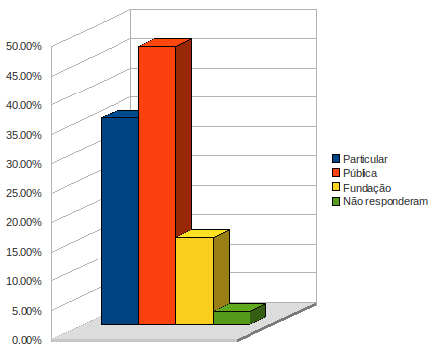
\includegraphics[width=0.7\linewidth]{arquivos/escola.png}
      \end{center}
      \caption{Tipo de escola dos participantes}
      \label{escola}
  \end{figure}

  Para ter um perfil etário de possíveis usuários do sistema, foi feito um levantamento dos tipos de participantes que responderam ao questionário. 
Segundo a figura~\ref{participante}, cerca de 70\% dos potenciais usuários são jovens com até 25 anos.

  \begin{figure}
      \begin{center}
	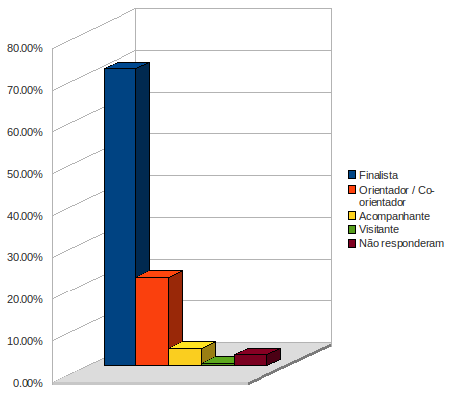
\includegraphics[width=0.7\linewidth]{arquivos/participante.png}
      \end{center}
      \caption{Tipo de participantes}
      \label{participante}
  \end{figure}

  A figura~\ref{local} mostra uma compilação da frequência de uso da internet em alguns locais. Pode-se constatar algumas coisas interessantes a partir 
da análise desse gráfico. É provável que os 12\% dos participantes que não acessam a Internet em casa não o façam por não ter acesso devido a 
condições financeiras, seja acesso discado ou banda larga, e é possível que nem possuam computador em casa. Mas dentre aqueles que possuem computador 
e acesso a internet, pode-se perceber que a frequência: quase 60\% dizem acessar a internet diaramente. Mais de 70\% dos participantes possuem 
acesso a Internet na escola, enquanto apenas cerca de 12\% não possuem acesso na escola, o que pode ser devido a não existir sala de informática 
ou à falta da conexão em si. É possível perceber que é baixa a frequencia de uso em espaços como lan houses e espaços públicos (nesse caso, foram 
considerados espaços públicos telecentros e bibliotecas; as escolas públicas não entraram), ou seja, menos de 10\% dos participantes fazem uso frequente 
desses locais para acessar a internet. 

  \begin{figure}
      \begin{center}
	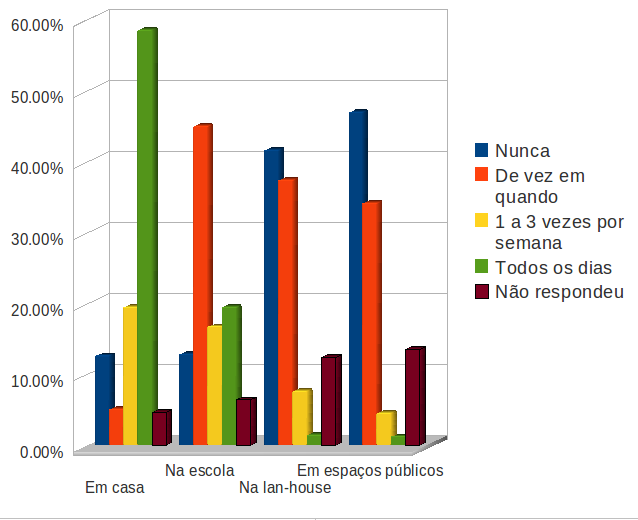
\includegraphics[width=0.7\linewidth]{arquivos/local.png}
      \end{center}
      \caption{Frequência de uso da Internet em locais}
      \label{local}
  \end{figure}

  Quanto aos aparelhos utilizados no acesso a internet, pode-se perceber pela figura~\ref{dispositivo} que a grande parcela dos acessos são feitos 
ainda por computadores \textit{desktop}, apesar de ter um número considerável de usuários de \textit{laptops}. Os dispositivos móveis, como celular 
e \textit{handhelds} possuem uma penetração ainda baixa; apenas cerca de 30\% dos participantes dizem já terem os usados para acessar 
a internet, sendo que mais da metade desse valor são de acessos esporádicos (de vez em quando).

  \begin{figure}
      \begin{center}
	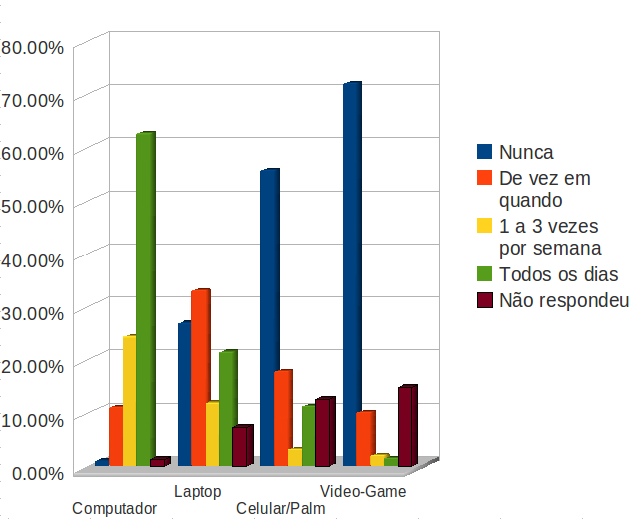
\includegraphics[width=0.7\linewidth]{arquivos/dispositivo.png}
      \end{center}
      \caption{Frequência de utilização de aparelhos para acesso a Internet}
      \label{dispositivo}
  \end{figure}

  Na figura~\ref{atividade}, percebe-se que o \textit{e-mail} é o serviço acesso que os participantes acessam com maior frequência: mais de 50\% 
faz uso dele diariamente. O segundo serviço mais acessado diariamente são os mensageiros instantâneos, como o MSN \textit{messenger} e o GTalk, 
com quase 40\%  das pessoas fazendo uso diário dele. Ao contrário do que é senso comum, as redes sociais são o quarto serviço em utilização diária 
com apenas pouco mais de 20\% dos participantes. Como pode-se constatar jogos, blogs, fóruns e chat possuem acesso esporádico entre os participantes 
da FEBRACE, sendo grande a porcentagem de pessoas que dizem nunca fazer uso deles. O acesso a vídeos, apesar de esporádico (com mais de 40\% das 
pessoas dizendo que usam "de vez em quando"), possui uma baixa porcentagem de participantes que não fazem uso desse serviço.

  \begin{figure}
      \begin{center}
	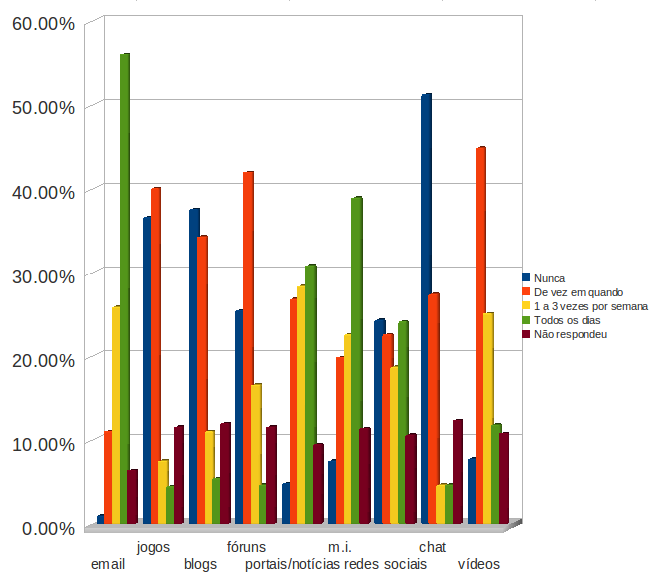
\includegraphics[width=0.7\linewidth]{arquivos/atividade.png}
      \end{center}
      \caption{Frequência de acesso a serviços na Internet}
      \label{atividade}
  \end{figure}

  Quanto às redes sociais mais usadas, segundo a figura~\ref{rede_social}, mais de 75\% dos participantes possuem conta na rede social Orkut, do 
Google. Em todas as demais, os participantes que as possuem não chega nem aos 10\%. Cerca de 15\% dos participantes afirmam não participar de redes 
sociais.

  \begin{figure}
      \begin{center}
	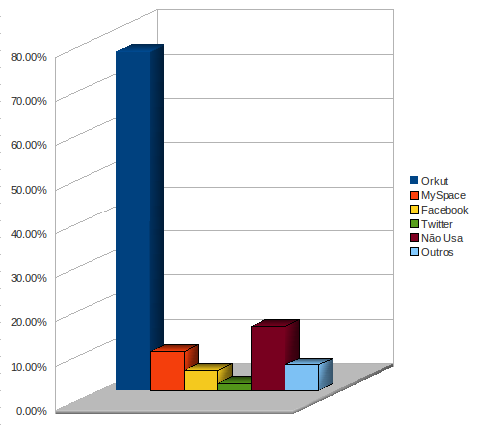
\includegraphics[width=0.7\linewidth]{arquivos/rede_social.png}
      \end{center}
      \caption{Redes Sociais mais utilizadas}
      \label{rede_social}
  \end{figure}

  Como pode-se ver na figura~\ref{contato} para mais de 85\% dos participantes é importante manter contato com os demais participantes da feira após 
seu término. Isso reforça a idéia que um espaço para o encontro desses participantes seria muito bem vindo.

  \begin{figure}
      \begin{center}
	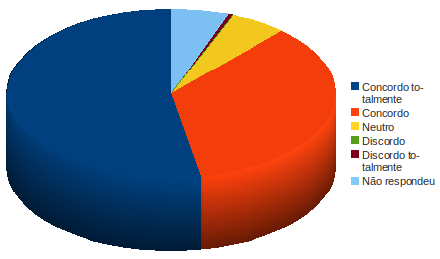
\includegraphics[width=0.7\linewidth]{arquivos/contato.png}
      \end{center}
      \caption{Participantes que acham importante poder manter contato com os outros da feira após o fim da Febrace}
      \label{contato}
  \end{figure}

  Mais de 60\% dos participantes, de acordo com a figura~\ref{feira_virtual}, acham que é possível que um grupo trabalhe num mesmo projeto sem 
estar na mesma cidade, através do uso da Internet. Apesar desse não ser o foco do atual projeto, mostra uma potencialidade para extensão no futuro, 
agregando funcionalidades que apóiem essa possibilidade.

  \begin{figure}
      \begin{center}
	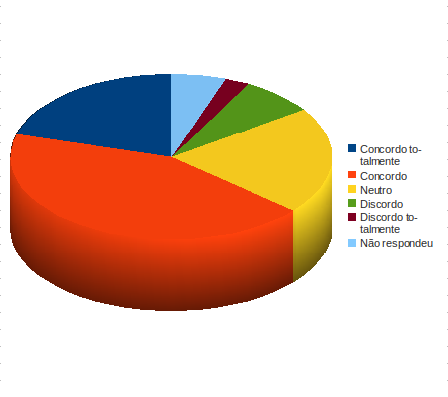
\includegraphics[width=0.7\linewidth]{arquivos/trabalho_online.png}
      \end{center}
      \caption{Participantes que acham possível um grupo trabalhar num mesmo projeto sem estar na mesma cidade, pela Internet}
      \label{trabalho_online}
  \end{figure}

  De acordo com figura~\ref{feira_virtual} mais de 60\% dos participantes acham que a idéia de uma feira de ciências virtual é interessante, enquanto 
apenas cerca de 10\% discordam da idéia. Isso reforça que a idéia do presente projeto apresenta relevância entre pessoas interessadas na temática.

  \begin{figure}
      \begin{center}
	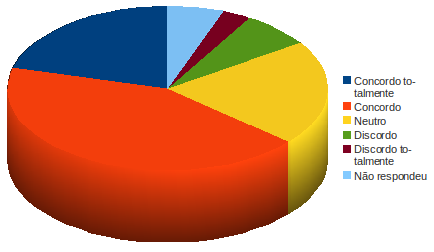
\includegraphics[width=0.7\linewidth]{arquivos/feira_virtual.png}
      \end{center}
      \caption{Participantes que acham a idéia de uma feira de ciências virtual na internet interessante}
      \label{feira_virtual}
  \end{figure}

\section{Levantamento de Histórias}

  O planejamento em XP feito com Histórias escritas em pequenos cartões. Cada cartão é escrito pelo cliente e deve descrever uma unidade de funcionalidade, que geralmente representa um requisito funcional desejado\cite{sato07}.

  Como uma forma de especificar o sistema a ser desenvolvido durante o projeto de formatura optou-se por descrever as histórias levantadas. As histórias foram escritas em conjunto com o cliente.

	\begin{enumerate}
    \item Convite a ex-participantes \\
      Quero, como administrador do sistema, que seja enviado automaticamente um convite para participação na rede social para todos os participantes de edições anteriores da FEBRACE (cadastrados em um banco de dados legado). Caso o ex-participante crie seu perfil na rede social, o projeto dele deve ser criado automaticamente e associado a ele.
    \item Autenticação no sistema \\
      Quero, como usuário, acessar a página inicial com meu e-mail e senha para me autenticar no sistema. Caso esqueça minha senha, quero informar o sistema e pedir que envie uma nova senha para meu e-mail. Se não for um usuário registrado, quero que me seja apresentada a tela de cadastro de novo usuário.
    \item Cadastro de Usuário \\
      Quero poder criar um perfil no sistema através de cadastro no sistema fornecendo um e-mail válido e uma senha para o acesso.
    \item Edição de Perfil \\
      Quero, como usuário registrado, poder editar a página de meu perfil pessoal, alterando, inserindo e excluindo os dados lá presentes, e escolhendo quais usuários podem ter acesso a determinadas informações minhas.
    \item Visualização de Perfil \\
      Quero, como usuário, poder visualizar meu perfil e de meus amigos, bem como, via sistema de busca, visualizar os perfis de quem o permita a qualquer usuário.
    \item Cancelamento de Cadastro \\
      Quero, como usuário, poder quando assim desejar cancelar meu cadastro do sistema.
    \item Visualização de Projeto \\
      Quero, como usuário, ver as informações de cada projeto, como seu nome e resumo, sua área do conhecimento, participantes e demais informações relevantes.
    \item Visualização de Participantes de um projeto \\
      Quero, como usuário, ver na página de um projeto quais são seus participantes, e ter acesso a seus perfis. Gostaria de saber também qual seu papel na Feira (estudante, orientador, etc.) e a instituição a qual pertence.
    \item Visualização de Vídeo de um projeto \\
      Quero, como usuário, poder ver na página de um projeto, quando disponível, seu vídeo oficial, feito na própria FEBRACE, hospedado em um site dedicado como a IPTV-USP ou o Youtube.
    \item Visualização de prêmios de um projeto \\
      Quero, como usuário, saber quais prêmios foram ganhos por algum projeto na edição da feira em que participou. Quero também poder acessar mais informações sobre esses prêmios.
    \item Edição dos Conteúdos de um projeto \\
      Quero, como participante de um projeto, poder inserir novas informações em sua página, como textos (relatório, diário de bordo, etc.), fotos e vídeos relacionados com ele, entre outros. Quero também poder editar esses conteúdos por mim adicionados, modificando-os ou apagando-os.
    \item Edição de Diário de Bordo de um projeto \\
      Quero que cada projeto tenha a ele associado uma ferramenta que permita a criação de um diário de bordo online, com o formato de \textit{weblog}.
    \item Adicionar amigos \\
      Quero, como usuário, escolher quais outros usuários são meus amigos, dando a eles permissão de me escrever mensagens, entre outras operações.
    \item Adicionar projetos prediletos \\
      Quero, como usuário, fazer uma lista de projetos que mais me chamaram atenção na feira. Quero poder fazer um comentário que justifique minha indicação, se assim o desejar.
    \item Postar em fórum \\
      Quero, como usuário, ter um espaço que permita postar perguntas que outros usuários possam responder, avisos, notícias e quaisquer outro tipo de texto relacionado.
    \item Comentar em caixas de comentários \\
      Quero, como usuário, poder deixar comentários nas diversas páginas da rede social, como projetos, artigos e diários de bordo. Caso eu tenha feito o comentário estando logado, ele deve ser identificado e deve haver um link para meu perfil nele. Comentários de visitantes podem ou não ser aceitos a critério de quem administra o conteúdo comentado.
    \item Enviar mensagens a outros usuários \\
      Quero, como usuário, enviar mensagens privadas de texto a outros usuários e receber mensagens enviadas por ele. Quero também poder escolher quais usuários podem ou não me escrever.
    \item Buscar conteúdos do sistema \\
      Quero, como usuário, ter acesso a  um sistema de busca que permita encontrar projetos pesquisando pelo seu nome, área de conhecimento, local de origem, integrantes, entre outros. Quero também poder usá-lo para encontrar outros usuários.
    \item Notificação de novos conteúdos \\
      Quero, como usuário, ser notificado caso novos conteúdos (entradas em Diários de Bordo, colunas, etc.) sejam criados na rede social.
    \item Visualização de Coluna da Equipe FEBRACE \\
      Quero, como usuário, uma área na rede social na qual possa ler textos escritos por pessoas ligadas a feira, como a equipe da FEBRACE, avaliadores, ex-participantes, etc.
    \item Interface de escrita de colunas \\
      Quero, como participante da equipe da Febrace ter acesso a uma interface no qual o texto das colunas possam ser criados e inseridos no sistema.
    \item Estatísticas do uso do sistema \\
      Quero, como usuário, ter um espaço no site no qual possa ver quais são os artigos mais lidos, os projetos mais visitados, os projetos que mais são escolhidos como prediletos, os usuários mais ativos, conteúdos mais acompanhados, etc.
    \item Interface Administrativa \\
      Quero, como administrador do sistema, uma interface auxiliar ao da rede social que permita a realização de tarefas administrativas.
    \item Moderação de conteúdos \\
      Quero, como usuário moderador, poder tirar do ar conteúdos impróprios postados por usuários. Quando um conteúdo for excluído ou editado, quero que o sistema envie uma mensagem para esse usuário informando o motivo dessa ação.
    \item Gerenciamento de Usuários \\
      Quero, como administrador do sistema, poder inserir usuários, modificar suas informações e excluí-los do sistema. Quero também editar permissões de cada usuário, determinando o tipo de uso que ele pode fazer do sistema.
    \item Gerenciamento de conteúdo \\
      Quero, como administrador do sistema, inserir, editar e excluir quaisquer conteúdos (como colunas e páginas de projeto).
    \item Estatísticas do sistema \\
      Quero, como administrador do sistema, ter uma página que indique quais são as páginas mais visitadas do site, os usuários mais ativos e as requisições que ocupam maior tempo de processamento do servidor.
    \item Visualização de Prêmios \\
      Quero, como usuário, saber quais prêmios foram oferecidos na FEBRACE, por qual empresa/instituição e a quais projetos. Quero assim que os projetos contemplados ofereçam um link para a página do respectivo prêmio, e quero encontrar nessa página mais informações sobre eles.
    \item Visualização de Instituições \\
      Quero, como usuário, que as diversas instituições ligadas à FEBRACE, como escolas, centros técnicos, patrocinadores, entre outros, tenham sua página no portal, contendo mais informações sobre elas.
    \item Cadastro de novo projeto \\
      Quero, como usuário registrado, poder cadastrar um novo projeto em andamento para ser submetido para a próxima edição da FEBRACE. Posso escolher a opção de criar um diário de bordo para meu projeto, além de poder convidar outras pessoas para participar do projeto criado.
	\end{enumerate}

  \subsection{1\textsuperscript{a} iteração}
    Antes do início de uma iteração é necessário que se definam quais serão as histórias a serem implementadas nesse ciclo de desenvolvimento. Essa escolha se dá por meio do \textit{Planning Game}, ou Jogo do Planejamento. No \textit{Planning Game}, desenvolvedores e clientes sentam-se juntos, e têm a frente o conjunto de histórias escritas até o momento. Os clientes definem a prioridade das histórias, enquanto os desenvolvedores definem a complexidade (dificuldade de implementação) de cada uma. Levando em consideração esses dois parâmetros, os envolvidos escolhem um subconjunto de histórias, cuja prioridade seja mais alta e cuja complexidade seja possível de lidar no período de desenvolvimento. Assim definem-se as histórias a serem trabalhadas em uma iteração.

    Através do \textit{Planning Game} realizado com o cliente foi definida a primeira iteração do projeto. Fazem parte da primeira iteração as seguintes histórias:

    \begin{itemize}
      \item Autenticação no sistema
      \item Cadastro de usuário
      \item Visualização de Projeto
      \item Visualização de Participantes de um projeto
      \item Edição dos Conteúdos de um projeto
      \item Cadastro de novo projeto
    \end{itemize}

    A duração de cada iteração será de três semanas e após esse período será feita uma entrega para o cliente que avaliará os resultados obtidos e definirá a iteração seguinte.

\section{Tecnologias utilizadas}

  O projeto será desenvolvido em plataforma Linux, usando o servidor web Apache. A linguagem de programação escolhida foi o Python, com o uso do framework Django para a construção de aplicações web. Serão usadas ferramentas para teste automatizado de código como o PyUnit, o Twil e o Selenium. Uma possibilidade levantada pelo grupo é a do uso de componentes reusáveis do Django Plugables. O banco de dados a ser utilizado ainda está em aberto, sendo que para se decidir serão testados os desempenhos dos bancos de dados MySQL e PostgreSQL.

  O código do projeto será gerenciado por meio de um sistema descentralizado de controle de versões, o Git. Como será produzido um sistema com código fonte aberto, o mesmo será disponibilizado no GitHub, onde o projeto já se encontra hospedado\footnote{http://www.github.com/nathaliaspatricio/febracev}. Como forma de registro do andamento do projeto foi criado um blog\footnote{http://febracev.wordpress.com} para o mesmo no Wordpress, e para a compilação de referências bibliográficas estão sendo usados um disco virtual\footnote{http://febracev.4shared.com} e o CiteULike\footnote{http://www.citeulike.org/groupfunc/9663} da Springer. Como uma forma de ajudar no gerenciamento do projeto está sendo usado o site Producteev, e para a coleta e relato de \textit{bugs} será usado o Trac\footnote{http://www.lsi.usp.br/nate/trac}. Para fazer a compilação dos dados coletados com os questionários de perfil de uso está sendo usado o LimeSurvey\footnote{http://www.lsi.usp.br/nate/febracev}.

  As tecnologias foram escolhidas com base na experiência prévia e habilidades técnicas da equipe.

\section{Arquitetura do sistema}

  Como consequência do uso do framework para desenvolvimento web Django, a arquitetura do sistema deverá ser aquela especificada pelo Django.

  O Django usa uma arquitetura conhecida como MTV (Model, Template, View) que nada mais é que uma variação do modelo MVC (Model, View, Controller). No MVC, separam-se as regras de negócios (Controller), os dados e métodos de acessos aos mesmos (Model) e as regras de apresentação (View).

  No caso da arquitetura MTV, o framework Django é o que faz as vezes de controlador da arquitetura MVC. Sendo assim, na arquitetura MTV, o Controller não é responsável pela lógica do negócio e sim pelo funcionamento do sistema. Além de models, views e templates, no Django há também url dispatchers, middlewares e handlers e são estes que são encarados como Controller.

  No Model, são escritas as classes que designarão as tabelas no banco de dados. A manipulação dessas tabelas ocorre através do ORM (mapeamento objeto relacional) e, por isso, não é necessária a escrita de querys em SQL para a persistência dos dados. Uma outra vantagem é baixa preocupação com qual sistema gerenciador de banco de dados será usado, uma vez que o ORM suporta vários sistemas.

  Na camada Model também devem ser escritas as regras de acesso às informações, regras para os eventos de cada modelo (métodos save, delete, etc.), e também regras genéricas para eventos que podem ser usados em mais de um modelo (signals). Toda a lógica de manipulação da informação de uma aplicação estará em seu Model.

  Na camada View, são escritas as regras de negócio e as regras de apresentação do sistema.

  Na camada Template é definida a forma de apresentação dos dados que a View envia. Com o sistema de templates do Django é possível criar heranças, ou seja, um template base contendo a estrutura básica do sistema e templates específicos que herdam as características deste template base e atribuem/criam suas próprias características.

  Com o uso do framework Django, um projeto é um conjunto de aplicações. Uma Aplicação é uma determinada funcionalidade que compõe um projeto. Por causa disso, há a idéia de aplicações plugáveis no Django que é uma aplicação que pode ser usada em mais de um projeto com nenhuma ou quase nenhuma alteração de código. Isso quer dizer que a aplicação deve ter seus próprios Models, suas próprias Views, seus próprios Templates e encapsular o máximo possível de código que não se enquadre em um desses elementos.

  Tendo em vista essa arquitetura, espera-se ao longo do primeiro semestre desenvolver a primeira versão do projeto. Essa primeira versão contemplará as seguintes aplicações:

  \subsection{Projetos}
    O principal módulo da aplicação é o de projetos. Nele são reunidas e apresentadas ao público informações sobre um projeto, como, entre outras, descrição, autores, orientadores e região de origem. O módulo de projetos deve oferecer integração com um serviço de vídeo sob demanda (como o IPTV-USP), onde serão armazenados vídeos dos projetos. São nas páginas geradas por esse módulo que ocorrem a maior parte das interações entre os usuários, pois dão acesso aos módulos de comentários e mensagens.

  \subsection{Perfis}
    Cada usuário tem seu perfil na aplicação com suas informações pessoais. Esse módulo tem a função de gerir a apresentação desses perfis bem como oferecer as funcionalidades de edição e exclusão.

  \subsection{Comentários}
    Várias das páginas geradas pela aplicação, tais como as de projeto e de artigos, têm agregadas caixas de comentários que podem ser usadas pelos visitantes (cadastrados ou não). Esse módulo oferece essa funcionalidade.

  \subsection{Fórum}
    Pelas páginas geradas por esse módulo os usuários podem perguntar e responder uns aos outros questões relacionadas à feira e aos seus projetos. O fórum será composto por diversas áreas, cada uma relativa à área de conhecimento correspondente na Feira.

  \subsection{Blog}
    Esse módulo oferece, atrelado a cada projeto, uma ferramenta de Blog, ou Diário de Bordo virtual, na qual os participantes podem relatar o processo do desenvolvimento de seus projetos, sua experiência na feira ou qualquer outro assunto que achem pertinentes. Os blogs, tais como outros serviços de módulos com conteúdos dinâmicos, devem prover serviço de RSS.

  \subsection{Mensagens}
    Os usuários registrados podem enviar mensagens privadas a outros usuários, e esse módulo oferece essa funcionalidade. Haverá também um sistema de mensagens públicas (\textit{scrap}).

  \subsection{Colunas}
    O módulo de colunas possibilita a inserção de conteúdo proveniente da equipe da FEBRACE ou de seus colaboradores, em páginas com esse fim.

  \subsection{Busca}
    Além do acesso ao conteúdo da aplicação pelos menus correspondentes, é possível filtrá-lo por palavras-chave na ferramenta de busca.

  \subsection{Login}
    Módulo no qual usuários registrados autenticam sua entrada, e os não registrados têm a oportunidade de criar uma conta.

  \subsection{Administração}
    Interface administrativa da aplicação, que permite operações de moderação, gerenciamento de usuários e conteúdo, etc.

\section{Atividades realizadas}
  As atividades realizadas nos últimos meses dividem-se em três grupos: 1) Compilação parcial dos questionários para levantamento do perfil do público-alvo do projeto, 2) Fase de exploração do Febrace\textsuperscript{V} e 3) Implementação da primeira iteração. Essas atividades são descritas a seguir.

  \subsection{Compilação parcial dos questionários}
    Durante a última edição da FEBRACE, foram distribuídos cerca de 1000 questionários para seus participantes, e seu preenchimento era facultativo. Foram preenchidos, ao todo, 520 questionários. Esses dados estão sendo inseridos aos poucos na ferramenta \textit{LimeSurvey}, e no presente momento já foram processados 126 questionários.

  \subsection{Fase de exploração}
    A primeira fase de um projeto de XP é a fase de exploração\cite{beck04}, que abrange a tomada inicial de histórias, o levantamento inicial de aspectos relativos à arquitetura do sistema a ser desenvolvido e a escolha e familiarização com as tecnologias a serem utilizadas no projeto.
    A fase de exploração do Febrace\textsuperscript{V} ocorreu nas três primeiras semanas de abril, e nela foram realizadas as seguintes atividades:

    \begin{itemize}
      \item
        Levantamento das histórias do projeto;
      \item
        Definição da arquitetura do projeto;
      \item
        Escolha das tecnologias utilizadas;
      \item
        Realização do primeiro \textit{Planning game}
    \end{itemize}

    A descrição dessas atividades encontra-se nas seções anteriores.

  \subsection{Primeira iteração}
    A primeira iteração, com duração de três semanas, foi realizada entre 20 de abril e 8 de maio, teve como resultado a implementação de cinco histórias. A descrição de cada uma delas é feita abaixo.

    \subsubsection{História 2 - Autenticação no sistema}
      Parte do código do módulo de Login deve oferecer a funcionalidade de autenticação no sistema. Foram desenvolvidas as telas de \textit{login} e \textit{logout} do Febrace\textsuperscript{V}, e a elas foi integrada a lógica de autenticação de usuários e o mecanismo de validação de sessões.

    \subsubsection{História 3 - Cadastro de usuário}
      A segunda parte do módulo de Login é o cadastro de usuários. Para se cadastrar, o usuário deve entrar com seu nome de usuário desejado e senha, além de um email válido. Ao término do cadastro, um email é enviado para o usuário. Ele deve então clicar no link presente nesse email para ativar sua conta. Sua chave de ativação é válida por sete dias.

    \subsubsection{História 4 - Edição de perfil}
      Após a realização do cadastro, na primeira vez que o usuário entra no sistema ele tem opção de completar sua página de perfil. A edição do perfil não precisa ser realizada naquele momento, uma vez que qualquer usuário logado no sistema pode visualizar e alterar as informações presentes em seu perfil.

    \subsubsection{História 5 - Visualização de perfil}
      Cada usuário do sistema tem uma página pessoal, com seu perfil. Essa página pode ser acessada por qualquer visitante do Febrace\textsuperscript{V}, anônimo ou não. Posteriormente será criada a funcionalidade da alteração dos níveis de exibição dos dados do perfil (configuração de privacidade).

    \subsubsection{História 22 - Interface administrativa}
      Foi ativada a interface administrativa, que permite o gerenciamento de usuários e conteúdos do Febrace\textsuperscript{V}.

    No segundo \textit{Planning Game}, programado para ocorrer no dia 11 de maio, serão definidas as histórias que serão desenvolvidas na segunda iteração.
